% Template for final reports and dissertations (Instituto Politécnico de Beja)
% Author: João Paulo Barros, joao.barros@ipbeja.pt

%para texto em Português PT
%para texto em Inglês substitua PT por EN
\documentclass[PT,alphabetic]{ipbeja-format}
%\documentclass[EN,alphabetic]{ipbeja-format}
% Para preencher 

\newcommand{\ESCOLA}{<<Nome da Escola>>}
%\newcommand{\ESCOLA}{Escola Superior de Tecnologia e Gestão}
%\newcommand{\ESCOLA}{Escola Superior de Educação}
%\newcommand{\ESCOLA}{Escola Superior Agrária}
%\newcommand{\ESCOLA}{Escola Superior de Saúde}


%\newcommand{\CURSO}{Licenciatura/Mestrado/... em ...}

\newcommand{\TITULO}{<<Título>>}

% Se pretender subtítulo
\newcommand{\SUBTITULO}{Opcionalmente, colocar aqui sub-título com máximo de vinte palavras}
% Se NÃO pretender subtítulo retire o % (comentário) da linha seguinte e coloque na linha anterior
%\newcommand{\SUBTITULO}{} 

\newcommand{\NOMEALUNO}{<<Nome Completo Estudante>>}

\newcommand{\DECLARACAO}{<<Dissertação apresentada ao instituto politécnico de beja para obtenção do grau de mestre em xx, ramo de xx>>}

\newcommand{\LOCAL}{<<LOCAL>>}
\newcommand{\MES}{<<MES>>}
\newcommand{\ANO}{<<ANO>>}


\newcommand{\orientacao}{ORIENTAÇÃO}
\newcommand{\nomesorientacao}{Colocar o título e nome de ou dois orientadores, por exemplo "Professora Doutora Nome Completo ou Abreviado\\Eng. Nome Completo ou Abreviado".}

% se não existir supervisor (docente do IPBeja, com orientador noutra entidade, colocar comentários nas linhas seguintes
\newcommand{\supervisao}{SUPERVISÃO}
\newcommand{\nomesupervisao}{Colocar o título e nome do supervidor, por exemplo "Professora Doutora Nome Completo ou Abreviado"}

%\input{02-info-to-fill-EN}
\usepackage[]{hyperref}
\hypersetup{hidelinks,hypertexnames=true}

\begin{document}
\setcounter{page}{1}
\thispagestyle{empty} 
\input{parte-inicial/capa} 
\pagestyle{ruled} 

\input{parte-inicial/folhaRosto}
\tituloPretextual{Resumo}

Este relatório apresenta o desenvolvimento de uma solução de automação para serviços de Administração de Sistemas em Linux, no âmbito da unidade curricular de Administração de Sistemas (2025/2026). O trabalho tem como objetivo reduzir tarefas manuais de configuração e promover maior consistência operacional através de scripts executados num servidor Linux virtualizado em VirtualBox. A solução contempla a automatização de operações sobre DNS, integração com serviços Web, gestão de partilhas de rede e procedimentos de apoio à administração, incluindo mecanismos de segurança e de backup. O projeto segue uma abordagem incremental, com validação funcional em ambiente de laboratório, recorrendo a uma máquina cliente para testes de conectividade e de acesso aos serviços disponibilizados. Para além da implementação técnica, o relatório sistematiza decisões de configuração, procedimentos de execução e critérios de verificação, constituindo um manual de referência para reprodução e manutenção do sistema.

\textbf{Palavras-chave}: administração de sistemas, Linux, automação, scripts, DNS, serviços de rede, segurança, backups.

\tituloPretextual{Abstract}


This report presents the development of an automation solution for Linux System Administration services, within the scope of the System Administration course (2025/2026). The main goal is to reduce manual configuration tasks and improve operational consistency through scripts executed on a Linux server virtualized in VirtualBox. The solution covers automated operations for DNS management, Web service integration, network share administration, and support procedures related to security and backup activities. The project follows an incremental development approach and includes functional validation in a laboratory environment, using a client machine to test connectivity and service availability. In addition to the technical implementation, the report documents configuration decisions, execution procedures, and verification criteria, so that the implemented solution can be reproduced, maintained, and evolved throughout the project lifecycle.

\textbf{Keywords}: system administration, Linux, automation, scripting, DNS, network services, security, backups.


%Opcional
%\input{parte-inicial/agradecimentos}

\indicegeral  
\indicedefiguras % Remover se houver menos de 5 figuras
\indicedetabelas % Remover se houver menos de 5 tabelas
\indicedelistagens % Remover se houver menos de 5 listagens
% Opcional
%\include{parte-inicial/abreviaturas} 
% Opcional
%\include{parte-inicial/simbologiaENotacoes} 

%%%%%%%%%%%%%%%%%%%%%%%%%%%%%%%%%%%%%%%%%%%%


\chapter{Introdução}
\label{intro}

No âmbito da unidade curricular de Administração de Sistemas, foi proposto o desenvolvimento de um projeto orientado à automatização da configuração de serviços num servidor Linux. O enunciado define um conjunto de funcionalidades técnicas centradas na gestão de DNS, integração com serviços Web, administração de partilhas de rede, mecanismos de backup e reforço da segurança do sistema, privilegiando sempre a execução automática por scripts.

Este trabalho surge da necessidade de reduzir tarefas manuais repetitivas que, em contextos de administração de sistemas, tendem a aumentar a probabilidade de erro, dificultar a normalização de configurações e tornar a manutenção mais morosa. Neste sentido, a automação é assumida como estratégia principal para melhorar a eficiência operacional, garantir maior consistência entre configurações e facilitar a reprodução dos procedimentos técnicos em diferentes momentos de execução.

O objetivo geral consiste em implementar uma solução capaz de configurar e gerir, de forma automatizada, um conjunto de serviços de administração de sistemas em Linux, com validação em ambiente virtualizado. O desenvolvimento é realizado com recurso a, pelo menos, uma máquina servidor Linux e uma máquina cliente para testes, ambas em VirtualBox, em conformidade com os requisitos do projeto.

Ao longo do relatório serão apresentados, de forma progressiva, o enquadramento técnico das opções adotadas, as etapas de implementação e os resultados de validação. A estrutura do documento segue uma lógica de desenvolvimento que inclui a descrição detalhada dos procedimentos técnicos, a análise crítica das soluções implementadas e a reflexão sobre os desafios enfrentados durante o processo de automação.
 % capitulo 1
\chapter{Arquitetura e ambiente de testes}
\label{cap2}

Este capítulo descreve o ambiente laboratorial utilizado para o desenvolvimento e validação do projeto, incluindo a infraestrutura virtualizada, a organização cliente-servidor, a stack técnica adotada e os principais critérios de teste. O objetivo deste ambiente foi garantir condições controladas para instalar, configurar e verificar de forma automatizada os serviços de Administração de Sistemas previstos no enunciado.

O laboratório foi implementado em Oracle VM VirtualBox, sobre um computador anfitrião com sistema operativo Windows, que também foi utilizado como plataforma complementar de teste em algumas etapas. A opção por virtualização permitiu repetir configurações, isolar o contexto de execução e reduzir riscos sobre o sistema anfitrião, mantendo simultaneamente flexibilidade para reconfiguração durante o desenvolvimento.

Foram utilizadas duas máquinas virtuais principais, ambas com AlmaLinux 8. A máquina \textit{AS\_Server} foi configurada como servidor central do projeto, com disco principal de 20 GB e três discos adicionais de 5 GB destinados à implementação de RAID 5. A máquina \textit{AS\_Client}, também com AlmaLinux 8, e disco de 20 GB, foi utilizada para testar os serviços disponibilizados pelo servidor. Em ambos os casos foi selecionado no VirtualBox o tipo Linux e o subtipo Red Hat (64-bit)

A conetividade entre as máquinas foi definida em modo \textit{Bridged Adapter}, esta escolha permitiu que as máquinas virtuais se comportassem como nós autónomos na rede local, com comunicação direta entre cliente e servidor e acesso à Internet para instalação de pacotes e dependências. Importa salientar que o endereçamento IP não foi fixo e variaram consoante a rede onde o laboratório era executado.

Após a instalação base do sistema operativo nas duas VMs, foram aplicadas configurações iniciais de preparação do ambiente: atualização do sistema, instalação de pacotes essenciais, ajuste de hostname, preparação de acesso remoto por SSH e criação da diretoria de trabalho para os scripts (\texttt{/root/projeto}). Para acelerar a fase inicial de validação laboratorial e reduzir interferências externas, foram também adotadas medidas de simplificação temporária, nomeadamente desativação de SELinux e da \textit{firewalld}.

Do ponto de vista de implementação, o projeto foi desenvolvido  em Bash, por oferecer integração direta com ferramentas nativas de administração Linux e boa adequação à automatização de tarefas sequenciais. A stack técnica incluiu os serviços e utilitários necessários para cobrir os requisitos do enunciado: BIND/named para DNS, Apache httpd para serviço Web e VirtualHosts, Samba para partilhas com clientes Windows, NFS para partilhas com clientes Linux/Unix, \texttt{tar} e \texttt{rsync} para backups, \texttt{mdadm} para RAID 5, Fail2Ban para mitigação de ataques de força bruta a SSH. 

Em síntese, a arquitetura adotada privilegiou simplicidade, repetibilidade e alinhamento com os requisitos do projeto. Embora o ambiente tenha sido desenhado para fins laboratoriais e académicos, com algumas simplificações controladas de segurança em fases iniciais, a sua estrutura permitiu suportar com eficácia o desenvolvimento dos scripts, a demonstração dos serviços e a produção de evidências técnicas para o relatório final.



\chapter{Automa\c{c}\~ao DNS e Web}
\label{cap3}

\section{Enquadramento do cap\'{\i}tulo}

Este cap\'{\i}tulo apresenta a implementa\c{c}\~ao dos pontos do enunciado associados \`a administra\c{c}\~ao de DNS e de servi\c{c}os Web, com foco na automatiza\c{c}\~ao de tarefas operacionais que, quando feitas manualmente, s\~ao mais demoradas e propensas a erro.

Do ponto de vista funcional, o DNS (\textit{Domain Name System}) garante a resolu\c{c}\~ao de nomes para endere\c{c}os IP. Isso permite que os servi\c{c}os sejam acedidos por dom\'{\i}nios leg\'{\i}veis em vez de endere\c{c}os num\'ericos. J\'a o servi\c{c}o Web, neste caso com Apache (\texttt{httpd}), responde aos pedidos HTTP e entrega o conte\'udo definido para cada dom\'{\i}nio atrav\'es de \textit{VirtualHosts}.

No contexto do projeto, estas duas camadas est\~ao diretamente ligadas: primeiro o DNS aponta o dom\'{\i}nio para o servidor, depois o Apache seleciona o \textit{VirtualHost} correto para servir a p\'agina esperada. Por isso, a integra\c{c}\~ao DNS+Web \'{e} tratada aqui de forma conjunta, com valida\c{c}\~ao em ambiente cliente-servidor.

\section{Quest\~ao 1: cria\c{c}\~ao autom\'atica de zona master DNS}
\label{sec:q1}

\subsection{Objetivo}

Na Quest\~ao 1, pretende-se automatizar a cria\c{c}\~ao de uma zona \textit{master} no servidor DNS, a partir da introdu\c{c}\~ao, por parte do utilizador, do nome do dom\'{\i}nio e do endere\c{c}o IP do servidor. O objetivo principal consiste em eliminar a necessidade de configura\c{c}\~ao manual no BIND, assegurando que a nova zona \'{e} criada de forma autom\'atica e que inclui, pelo menos, os registos do tipo \texttt{A} necess\'arios para a resolu\c{c}\~ao do dom\'{\i}nio para o IP do servidor DNS/Web.

Esta automatiza\c{c}\~ao permite reduzir erros de configura\c{c}\~ao, tornar o processo mais r\'apido e garantir uma estrutura uniforme na cria\c{c}\~ao de novas zonas DNS.

\subsection{Prepara\c{c}\~ao do servi\c{c}o DNS}

Antes da execu\c{c}\~ao do script, foi necess\'ario preparar a m\'aquina servidor com os pacotes e servi\c{c}os base do BIND, de forma a disponibilizar o ambiente necess\'ario \`a cria\c{c}\~ao e valida\c{c}\~ao das zonas DNS.

\begin{lstlisting}[language=bash,caption={Preparacao inicial do servico DNS}]
yum install bind bind-utils -y
systemctl enable named
systemctl start named
systemctl status named
\end{lstlisting}

Foram instalados os pacotes \texttt{bind} e \texttt{bind-utils}, essenciais para o servi\c{c}o DNS e para a valida\c{c}\~ao de configura\c{c}\~oes. Em seguida, o servi\c{c}o \texttt{named} foi ativado e iniciado, garantindo que o servidor estava operacional antes da execu\c{c}\~ao do script.

Ap\'os a instala\c{c}\~ao e ativa\c{c}\~ao do servi\c{c}o, foi criada a diretoria de trabalho do projeto, onde foram armazenados os scripts desenvolvidos ao longo da implementa\c{c}\~ao.

\begin{lstlisting}[language=bash,caption={Criacao da diretoria de trabalho}]
mkdir -p /root/projeto
cd /root/projeto
\end{lstlisting}

A cria\c{c}\~ao desta diretoria permitiu centralizar os scripts do projeto num local \'unico, facilitando execu\c{c}\~ao, manuten\c{c}\~ao e testes.

\subsection{Implementa\c{c}\~ao do script}

O script \texttt{q1\_dns.sh} automatiza a cria\c{c}\~ao da zona \textit{master} DNS a partir do dom\'{\i}nio e do IP introduzidos pelo utilizador. O fluxo foi organizado em blocos: defini\c{c}\~oes iniciais, valida\c{c}\~oes, integra\c{c}\~ao no BIND, cria\c{c}\~ao da zona e valida\c{c}\~ao final.

\begin{lstlisting}[language=bash,caption={Definicoes base e validacoes iniciais}]
MAINCONF="/etc/named.conf"
CONFZONES="/etc/named/zones.conf"
ZONEDIR="/var/named"

read -p "Introduza o nome do dominio: " DOMINIO
read -p "Introduza o IP do servidor DNS/Web: " IP

if [ "$EUID" -ne 0 ]; then
    echo "Erro: execute como root."
    exit 1
fi
\end{lstlisting}

Este bloco define a base da solu\c{c}\~ao e valida a execu\c{c}\~ao como \texttt{root}, condi\c{c}\~ao necess\'aria para alterar ficheiros de sistema.

De seguida, s\~ao feitas valida\c{c}\~oes para garantir que dom\'{\i}nio, IP, pacotes e caminhos necess\'arios est\~ao dispon\'{\i}veis.

\begin{lstlisting}[language=bash,caption={Validacao de pre-condicoes de execucao}]
if [ -z "$DOMINIO" ] || [ -z "$IP" ]; then
    echo "Erro: dominio e IP sao obrigatorios."
    exit 1
fi

if ! command -v named-checkconf >/dev/null 2>&1; then
    echo "Erro: BIND/DNS nao esta instalado."
    echo "Execute: yum install bind bind-utils -y"
    exit 1
fi

if [ ! -f "$MAINCONF" ]; then
    echo "Erro: ficheiro $MAINCONF nao existe."
    exit 1
fi

if [ ! -d "$ZONEDIR" ]; then
    echo "Erro: diretoria $ZONEDIR nao existe."
    exit 1
fi
\end{lstlisting}

Estas verifica\c{c}\~oes evitam configura\c{c}\~oes incompletas e paragens por erro em ambiente n\~ao preparado.

Numa segunda fase, o script integra a nova zona no BIND atrav\'es do ficheiro \texttt{/etc/named/zones.conf}, evitando altera\c{c}\~oes repetidas no \texttt{named.conf}.

\begin{lstlisting}[language=bash,caption={Integracao da zona e prevencao de duplicados}]
touch "$CONFZONES"

if ! grep -q 'include "/etc/named/zones.conf";' "$MAINCONF"; then
    echo '' >> "$MAINCONF"
    echo 'include "/etc/named/zones.conf";' >> "$MAINCONF"
fi

if grep -q "zone \"$DOMINIO\"" "$CONFZONES"; then
    echo "Erro: a zona $DOMINIO ja existe em $CONFZONES"
    exit 1
fi

if [ -f "$ZONEFILE" ]; then
    echo "Erro: o ficheiro $ZONEFILE ja existe."
    exit 1
fi
\end{lstlisting}

Este bloco impede duplica\c{c}\~oes e torna o processo de cria\c{c}\~ao de zonas mais robusto.

Numa terceira fase, o script cria o ficheiro de zona com os registos m\'{\i}nimos (\texttt{SOA}, \texttt{NS} e \texttt{A}).

\begin{lstlisting}[language=bash,caption={Criacao do ficheiro de zona}]
cat > "$ZONEFILE" <<EOF
\$TTL 86400
@   IN  SOA ns1.$DOMINIO. root.$DOMINIO. (
        $SERIAL ; serial
        3600    ; refresh
        1800    ; retry
        604800  ; expire
        86400 ) ; minimum

@       IN  NS  ns1.$DOMINIO.
@       IN  A   $IP
ns1     IN  A   $IP
www     IN  A   $IP
EOF
\end{lstlisting}

Este \'e o n\'ucleo funcional do script, pois garante a gera\c{c}\~ao din\^amica da zona e o cumprimento do requisito de resolu\c{c}\~ao do dom\'{\i}nio para o IP indicado.

Ap\'os a cria\c{c}\~ao do ficheiro de zona, o script aplica permiss\~oes adequadas e regista formalmente a nova zona no ficheiro \texttt{zones.conf}.

\begin{lstlisting}[language=bash,caption={Permissoes e registo formal da nova zona}]
chown root:named "$ZONEFILE"
chmod 640 "$ZONEFILE"

cat >> "$CONFZONES" <<EOF

zone "$DOMINIO" IN {
    type master;
    file "$DOMINIO.zone";
    allow-update { none; };
};
EOF
\end{lstlisting}

A atribui\c{c}\~ao de permiss\~oes garante leitura correta pelo \texttt{named} e a entrada em \texttt{zones.conf} torna a zona ativa no BIND.

Por fim, o script valida toda a configura\c{c}\~ao antes de reiniciar o servi\c{c}o DNS.

\begin{lstlisting}[language=bash,caption={Validacao e ativacao da configuracao}]
named-checkconf || { echo "Erro no ficheiro $MAINCONF"; exit 1; }
named-checkzone "$DOMINIO" "$ZONEFILE" || { echo "Erro no ficheiro de zona"; exit 1; }
systemctl restart named
systemctl enable named
\end{lstlisting}

Este bloco confirma a validade da configura\c{c}\~ao antes de reiniciar o servi\c{c}o, reduzindo o risco de deixar o DNS em estado inconsistente.

\subsection{Execu\c{c}\~ao e demonstra\c{c}\~ao}

Ap\'os atribuir permiss\~ao de execu\c{c}\~ao ao script (\texttt{chmod +x /root/projeto/q1\_dns.sh}), a execu\c{c}\~ao foi conclu\'{\i}da com sucesso para o dom\'{\i}nio \texttt{teste.com}. A valida\c{c}\~ao confirmou a cria\c{c}\~ao do ficheiro de zona, o registo da zona em \texttt{/etc/named/zones.conf} e a resolu\c{c}\~ao correta no cliente.

\subsection{Evid\^encias visuais da Quest\~ao 1}

\begin{figure}[H]
\centering

\includegraphics[width=0.95\textwidth]{q1_execucao}
\caption{Execucao do script da Questao 1 e validacao da zona criada}
\label{fig:q1-execucao}
\end{figure}

\begin{figure}[H]
\centering

\includegraphics[width=0.95\textwidth]{q1_zonefile}
\caption{Conteudo do ficheiro de zona gerado automaticamente}
\label{fig:q1-zonefile}
\end{figure}

\begin{figure}[H]
\centering

\includegraphics[width=0.95\textwidth]{q1_zonesconf}
\caption{Definicao da zona adicionada em \texttt{/etc/named/zones.conf}}
\label{fig:q1-zonesconf}
\end{figure}

\begin{figure}[H]
\centering

\includegraphics[width=0.85\textwidth]{q1_nslookup_windows}
\caption{Validacao da resolucao DNS no cliente Windows}
\label{fig:q1-nslookup}
\end{figure}

\clearpage
\section{Quest\~ao 3: integra\c{c}\~ao DNS e VirtualHost Web}
\label{sec:q3}

\subsection{Objetivo}

A Quest\~ao 3 constitui uma extens\~ao direta da Quest\~ao 1. Para al\'em da cria\c{c}\~ao autom\'atica da zona DNS, o script passa tamb\'em a configurar automaticamente o servi\c{c}o Web, de forma a permitir que o dom\'{\i}nio criado responda por HTTP atrav\'es de um \textit{VirtualHost} dedicado no Apache.

Em termos pr\'aticos, a solu\c{c}\~ao implementada passa a abranger todo o ciclo de publica\c{c}\~ao de um dom\'{\i}nio, incluindo:

\begin{enumerate}
    \item cria\c{c}\~ao da zona DNS e do respetivo ficheiro de zona;
    \item cria\c{c}\~ao da diretoria Web associada ao dom\'{\i}nio;
    \item gera\c{c}\~ao autom\'atica do ficheiro de \textit{VirtualHost} no Apache;
    \item cria\c{c}\~ao de uma p\'agina inicial de boas-vindas;
    \item valida\c{c}\~ao e rein\'{\i}cio dos servi\c{c}os \texttt{named} e \texttt{httpd}.
\end{enumerate}

Com esta abordagem, o dom\'{\i}nio fica funcional de ponta a ponta: resolve em DNS e responde por HTTP com um \textit{VirtualHost} dedicado.

\subsection{Implementa\c{c}\~ao do script \texttt{q3\_dns\_web.sh}}

Numa primeira fase, o script define os caminhos principais utilizados tanto pelo BIND como pelo Apache.

\begin{lstlisting}[language=bash,caption={Variaveis principais para DNS e Apache}]
MAINCONF="/etc/named.conf"
CONFZONES="/etc/named/zones.conf"
ZONEDIR="/var/named"

HTTPD_CONF_DIR="/etc/httpd/conf.d"
WEBROOT_BASE="/var/www"
\end{lstlisting}

Estas vari\'aveis organizam a configura\c{c}\~ao de DNS e Web e tornam o script mais leg\'{\i}vel. Depois da recolha do dom\'{\i}nio e do IP, o script valida o ambiente, garante a inclus\~ao \'unica de \texttt{zones.conf} e impede duplica\c{c}\~oes de zona, ficheiro de zona e \textit{VirtualHost}.

Ap\'os estas valida\c{c}\~oes, o script cria a zona DNS e avan\c{c}a para a componente Web, gerando a diretoria do dom\'{\i}nio e a p\'agina inicial.

\begin{lstlisting}[language=bash,caption={Criacao automatica de WebRoot e pagina inicial}]
WEBROOT="$WEBROOT_BASE/${DOMINIO}"
mkdir -p "$WEBROOT"

cat > "$WEBROOT/index.html" <<EOF
<!DOCTYPE html>
<html lang="pt">
<head>
    <meta charset="UTF-8">
    <title>Bem-vindo a $DOMINIO</title>
</head>
<body>
    <h1>Bem-vindo ao dominio $DOMINIO</h1>
    <p>Este VirtualHost foi criado automaticamente.</p>
</body>
</html>
EOF
\end{lstlisting}

Este bloco prepara o conte\'udo Web m\'{\i}nimo do dom\'{\i}nio, permitindo validar imediatamente o funcionamento do \textit{VirtualHost}.

Depois de preparar a estrutura de conte\'udos, o script cria o ficheiro de \textit{VirtualHost} no Apache.

\begin{lstlisting}[language=bash,caption={Configuracao do VirtualHost no Apache}]
cat > "$VHOSTFILE" <<EOF
<VirtualHost *:80>
    ServerName $DOMINIO
    ServerAlias www.$DOMINIO
    DocumentRoot "$WEBROOT"

    <Directory "$WEBROOT">
        AllowOverride All
        Require all granted
    </Directory>

    ErrorLog /var/log/httpd/${DOMINIO}_error.log
    CustomLog /var/log/httpd/${DOMINIO}_access.log combined
</VirtualHost>
EOF
\end{lstlisting}

Este bloco integra o dom\'{\i}nio no Apache: \texttt{ServerName}/\texttt{ServerAlias} definem os nomes atendidos, \texttt{DocumentRoot} define o conte\'udo e os logs ficam separados por dom\'{\i}nio.

Por fim, o script valida as configura\c{c}\~oes dos dois servi\c{c}os antes de proceder \`a sua ativa\c{c}\~ao definitiva.

\begin{lstlisting}[language=bash,caption={Validacao final e reinicio dos servicos}]
named-checkconf || { echo "Erro no named.conf"; exit 1; }
named-checkzone "$DOMINIO" "$ZONEFILE" || { echo "Erro na zona DNS"; exit 1; }
httpd -t || { echo "Erro na configuracao Apache"; exit 1; }

systemctl restart named
systemctl restart httpd
\end{lstlisting}

Este bloco final valida DNS e Apache antes do rein\'{\i}cio dos servi\c{c}os, garantindo aplica\c{c}\~ao segura da configura\c{c}\~ao.

\subsection{Valida\c{c}\~ao funcional}

A valida\c{c}\~ao da Quest\~ao 3 foi feita em tr\^es n\'{\i}veis para confirmar o funcionamento das componentes DNS e Web.

\begin{enumerate}
    \item \textbf{Execu\c{c}\~ao do script no servidor}: confirma cria\c{c}\~ao do ficheiro de zona DNS, da entrada correspondente em \texttt{zones.conf}, do ficheiro de \textit{VirtualHost} no Apache, da diretoria Web do dom\'{\i}nio e da p\'agina inicial \texttt{index.html};
    \item \textbf{Resolu\c{c}\~ao DNS no cliente}: confirma que o dom\'{\i}nio configurado \'{e} corretamente resolvido para o endere\c{c}o IP do servidor;
    \item \textbf{Acesso HTTP no navegador}: confirma que o Apache entrega corretamente a p\'agina de boas-vindas criada automaticamente pelo script.
\end{enumerate}

\subsection{Evid\^encias visuais da Quest\~ao 3}

\begin{figure}[H]
\centering

\includegraphics[width=0.95\textwidth]{q3_execucao}
\caption{Execucao da Questao 3 no servidor}
\label{fig:q3-execucao}
\end{figure}

\begin{figure}[H]
\centering

\includegraphics[width=0.85\textwidth]{q3_nslookup_windows}
\caption{Validacao de resolucao DNS no cliente Windows}
\label{fig:q3-nslookup}
\end{figure}

\begin{figure}[H]
\centering

\includegraphics[width=0.95\textwidth]{q3_http_browser}
\caption{Acesso HTTP ao VirtualHost criado automaticamente}
\label{fig:q3-http}
\end{figure}

\chapter{Automa\c{c}\~ao DNS e Web (Parte II)}
\label{cap4}

\section{Enquadramento do cap\'{\i}tulo}

Este cap\'{\i}tulo d\'{a} continuidade \`a automa\c{c}\~ao DNS e Web, com foco em opera\c{c}\~oes de remo\c{c}\~ao controlada, manuten\c{c}\~ao e robustez operacional. S\~ao apresentados os pontos associados \`a elimina\c{c}\~ao de configura\c{c}\~oes (Quest\~ao 6) e \`as melhorias de administra\c{c}\~ao e seguran\c{c}a (Quest\~ao 8), ficando este cap\'{\i}tulo preparado para integrar tamb\'{e}m o ponto P13 e restantes refor\c{c}os de seguran\c{c}a.
\section{Quest\~ao 6: eliminac\~ao de zonas master, VirtualHosts e zonas reverse}
\label{sec:q6}

\subsection{Objetivo}

A Quest\~ao 6 introduz a capacidade de remo\c{c}\~ao autom\'atica de elementos previamente criados nas quest\~oes anteriores. Em vez de se limitar \`a cria\c{c}\~ao de configura\c{c}\~oes, a aplica\c{c}\~ao passa tamb\'em a suportar opera\c{c}\~oes de elimina\c{c}\~ao controlada de zonas DNS \textit{forward}, VirtualHosts Apache e zonas DNS \textit{reverse}.

Esta funcionalidade completa o ciclo de administra\c{c}\~ao, permitindo criar e remover configura\c{c}\~oes de forma coerente, sem deixar entradas residuais nos servi\c{c}os.

\subsection{Implementa\c{c}\~ao do script \texttt{q6\_remover.sh}}

O script \texttt{q6\_remover.sh} concentra num \'unico ponto as opera\c{c}\~oes de remo\c{c}\~ao relacionadas com DNS e Apache. A l\'ogica principal cobre tr\^es opera\c{c}\~oes:

\begin{enumerate}
    \item elimina\c{c}\~ao de zonas master \textit{forward};
    \item elimina\c{c}\~ao de VirtualHosts Apache;
    \item elimina\c{c}\~ao de zonas \textit{reverse}.
\end{enumerate}

\begin{lstlisting}[language=bash,caption={Estrutura base do script}]
CONFZONES="/etc/named/zones.conf"
ZONEDIR="/var/named"
HTTPD_CONF_DIR="/etc/httpd/conf.d"
WEBROOT_BASE="/var/www"
\end{lstlisting}

Estas vari\'aveis definem de forma expl\'icita os locais de configura\c{c}\~ao e dados onde o script atua.

\begin{lstlisting}[language=bash,caption={Remocao de blocos de zona no zones.conf}]
remover_bloco_zona() {
    local nomezona="$1"

    awk -v zona="$nomezona" '
    BEGIN {skip=0}
    $0 ~ "^[[:space:]]*zone \""zona"\"" {skip=1; next}
    skip==1 && $0 ~ /^[[:space:]]*};[[:space:]]*$/ {skip=0; next}
    skip==0 {print}
    ' "$CONFZONES" > /tmp/zones.conf.new && mv /tmp/zones.conf.new "$CONFZONES"
}
\end{lstlisting}

Esta fun\c{c}\~ao \'{e} o n\'ucleo da remo\c{c}\~ao DNS, pois elimina o bloco completo da zona no \texttt{zones.conf}, e n\~ao apenas uma linha isolada.

\begin{lstlisting}[language=bash,caption={Eliminacao de zonas master forward}]
eliminar_zona_forward() {
    read -p "Dominio da zona master a eliminar: " DOMINIO
    ZONEFILE="$ZONEDIR/${DOMINIO}.zone"

    if grep -q "zone \"$DOMINIO\"" "$CONFZONES"; then
        remover_bloco_zona "$DOMINIO"
    fi

    [ -f "$ZONEFILE" ] && rm -f "$ZONEFILE"

    named-checkconf || { echo "Erro na configuracao DNS."; exit 1; }
    systemctl restart named
}
\end{lstlisting}

Nesta opera\c{c}\~ao, a remo\c{c}\~ao s\'o fica completa quando s\~ao eliminados tanto o bloco da zona no \texttt{zones.conf} como o ficheiro \texttt{.zone} em \texttt{/var/named}.

\begin{lstlisting}[language=bash,caption={Eliminacao de VirtualHosts Apache}]
eliminar_virtualhost() {
    read -p "Dominio do VirtualHost a eliminar: " DOMINIO

    VHOSTFILE="$HTTPD_CONF_DIR/${DOMINIO}.conf"
    WEBROOT="$WEBROOT_BASE/${DOMINIO}"

    [ -f "$VHOSTFILE" ] && rm -f "$VHOSTFILE"

    read -p "Deseja apagar tambem a pasta web $WEBROOT ? (s/n): " OP
    if [ "$OP" = "s" ] || [ "$OP" = "S" ]; then
        [ -d "$WEBROOT" ] && rm -rf "$WEBROOT"
    fi

    httpd -t || { echo "Erro na configuracao Apache."; exit 1; }
    systemctl restart httpd
}
\end{lstlisting}

Este bloco remove o ficheiro de VirtualHost e, opcionalmente, a diretoria Web correspondente, permitindo uma remo\c{c}\~ao parcial ou completa conforme a necessidade.

\begin{lstlisting}[language=bash,caption={Eliminacao de zonas reverse}]
eliminar_zona_reverse() {
    read -p "Zona reverse a eliminar (ex: 2.50.10.in-addr.arpa): " REVZONE

    REVBASE=$(echo "$REVZONE" | sed 's/\.in-addr\.arpa//')
    REVFILE="$ZONEDIR/${REVBASE}.rev"

    if grep -q "zone \"$REVZONE\"" "$CONFZONES"; then
        remover_bloco_zona "$REVZONE"
    fi

    [ -f "$REVFILE" ] && rm -f "$REVFILE"

    named-checkconf || { echo "Erro na configuracao DNS."; exit 1; }
    systemctl restart named
}
\end{lstlisting}

Na remo\c{c}\~ao \textit{reverse}, o script converte primeiro a zona no formato \texttt{in-addr.arpa} para o nome base do ficheiro \texttt{.rev}, e depois aplica a mesma l\'ogica de consist\^encia usada nas zonas \textit{forward}.

\begin{lstlisting}[language=bash,caption={Menu de remocao}]
menu() {
    echo
    echo "===== MENU REMOCAO ====="
    echo "1 - Eliminar zona master (forward)"
    echo "2 - Eliminar VirtualHost"
    echo "3 - Eliminar zona reverse"
    echo "0 - Sair"
    echo
    read -p "Opcao: " OP

    case $OP in
        1) eliminar_zona_forward ;;
        2) eliminar_virtualhost ;;
        3) eliminar_zona_reverse ;;
        0) exit 0 ;;
        *) echo "Opcao invalida." ;;
    esac
}
\end{lstlisting}

O menu simplifica a utiliza\c{c}\~ao e centraliza as opera\c{c}\~oes de remo\c{c}\~ao num \'unico ponto.

\subsection{Valida\c{c}\~ao funcional}

A valida\c{c}\~ao foi realizada com execu\c{c}\~ao do script e verifica\c{c}\~ao dos ficheiros de configura\c{c}\~ao antes e depois das remo\c{c}\~oes.

\begin{lstlisting}[language=bash,caption={Execucao do script}]
chmod +x /root/projeto/q6_remover.sh
/root/projeto/q6_remover.sh
\end{lstlisting}

Foram testadas as tr\^es op\c{c}\~oes do menu: elimina\c{c}\~ao de zona \textit{forward}, elimina\c{c}\~ao de VirtualHost e elimina\c{c}\~ao de zona \textit{reverse}.

\begin{lstlisting}[language=bash,caption={Verificacao da remocao de VirtualHosts}]
ls /etc/httpd/conf.d
ls /var/www
httpd -t
\end{lstlisting}

\begin{lstlisting}[language=bash,caption={Verificacao da remocao de zonas DNS}]
cat /etc/named/zones.conf
ls /var/named
named-checkconf
\end{lstlisting}

Os testes confirmaram a remo\c{c}\~ao correta dos elementos selecionados e a manuten\c{c}\~ao da validade das configura\c{c}\~oes de DNS e Apache ap\'os cada opera\c{c}\~ao.

\subsection{Evid\^encias visuais da Quest\~ao 6}

\begin{figure}[!htbp]
\centering
\IfFileExists{figuras/q6_pre_www.png}{
  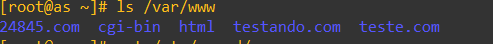
\includegraphics[width=0.78\textwidth,height=0.72\textheight,keepaspectratio]{figuras/q6_pre_www.png}
}{
  \fbox{\parbox{0.9\textwidth}{Inserir screenshot do estado inicial de \texttt{/var/www}.}}
}
\caption{Estado inicial da diretoria \texttt{/var/www}}
\label{fig:q6-pre-www}
\end{figure}

\begin{figure}[!htbp]
\centering
\IfFileExists{figuras/q6_pre_httpd_conf.png}{
  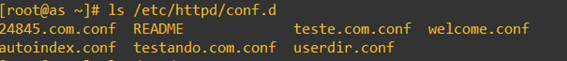
\includegraphics[width=0.78\textwidth,height=0.72\textheight,keepaspectratio]{figuras/q6_pre_httpd_conf.png}
}{
  \fbox{\parbox{0.9\textwidth}{Inserir screenshot do estado inicial de \texttt{/etc/httpd/conf.d}.}}
}
\caption{Estado inicial dos VirtualHosts em \texttt{/etc/httpd/conf.d}}
\label{fig:q6-pre-httpd}
\end{figure}

\begin{figure}[!htbp]
\centering
\IfFileExists{figuras/q6_pre_zones_conf.png}{
  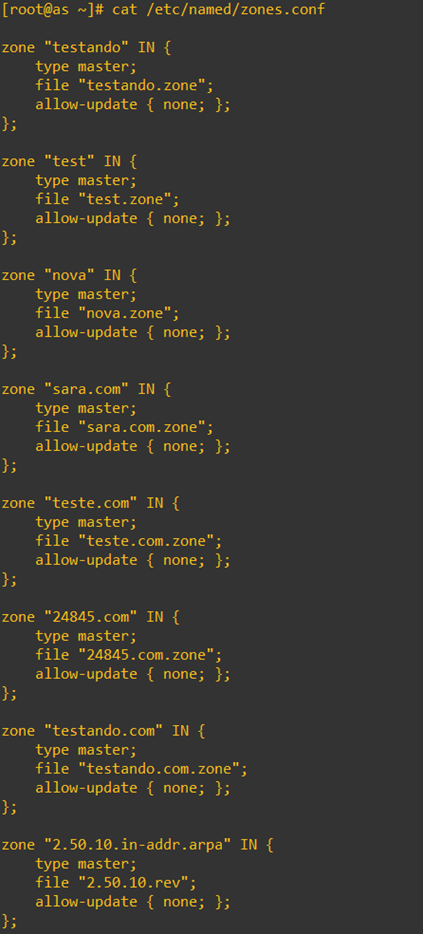
\includegraphics[width=0.78\textwidth,height=0.72\textheight,keepaspectratio]{figuras/q6_pre_zones_conf.png}
}{
  \fbox{\parbox{0.9\textwidth}{Inserir screenshot inicial de \texttt{/etc/named/zones.conf}.}}
}
\caption{Estado inicial do ficheiro \texttt{zones.conf}}
\label{fig:q6-pre-zones}
\end{figure}

\begin{figure}[!htbp]
\centering
\IfFileExists{figuras/q6_exec_forward.png}{
  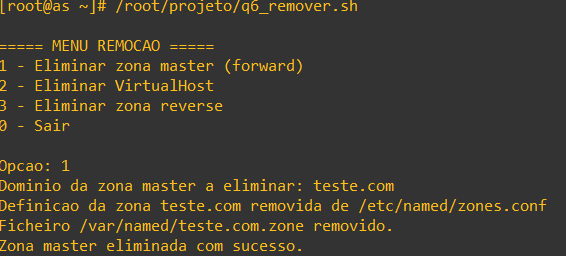
\includegraphics[width=0.78\textwidth,height=0.72\textheight,keepaspectratio]{figuras/q6_exec_forward.png}
}{
  \fbox{\parbox{0.9\textwidth}{Inserir screenshot da remocao de zona master (opcao 1).}}
}
\caption{Execucao da opcao de remocao de zona master forward}
\label{fig:q6-exec-forward}
\end{figure}

\begin{figure}[!htbp]
\centering
\IfFileExists{figuras/q6_exec_vhost.png}{
  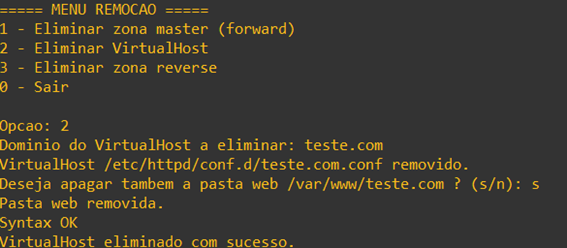
\includegraphics[width=0.78\textwidth,height=0.72\textheight,keepaspectratio]{figuras/q6_exec_vhost.png}
}{
  \fbox{\parbox{0.9\textwidth}{Inserir screenshot da remocao de VirtualHost (opcao 2).}}
}
\caption{Execucao da opcao de remocao de VirtualHost}
\label{fig:q6-exec-vhost}
\end{figure}

\begin{figure}[!htbp]
\centering
\IfFileExists{figuras/q6_exec_reverse.png}{
  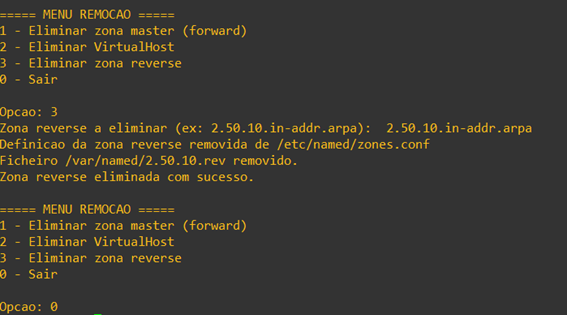
\includegraphics[width=0.78\textwidth,height=0.72\textheight,keepaspectratio]{figuras/q6_exec_reverse.png}
}{
  \fbox{\parbox{0.9\textwidth}{Inserir screenshot da remocao de zona reverse (opcao 3).}}
}
\caption{Execucao da opcao de remocao de zona reverse}
\label{fig:q6-exec-reverse}
\end{figure}

\begin{figure}[!htbp]
\centering
\IfFileExists{figuras/q6_pos_httpd_www.png}{
  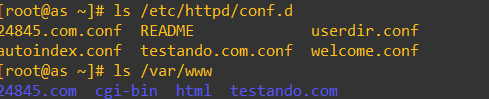
\includegraphics[width=0.78\textwidth,height=0.72\textheight,keepaspectratio]{figuras/q6_pos_httpd_www.png}
}{
  \fbox{\parbox{0.9\textwidth}{Inserir screenshot do estado final de \texttt{/etc/httpd/conf.d} e \texttt{/var/www}.}}
}
\caption{Estado final das estruturas Apache ap\'os remo\c{c}\~ao}
\label{fig:q6-pos-httpd}
\end{figure}

\begin{figure}[!htbp]
\centering
\IfFileExists{figuras/q6_pos_named.png}{
  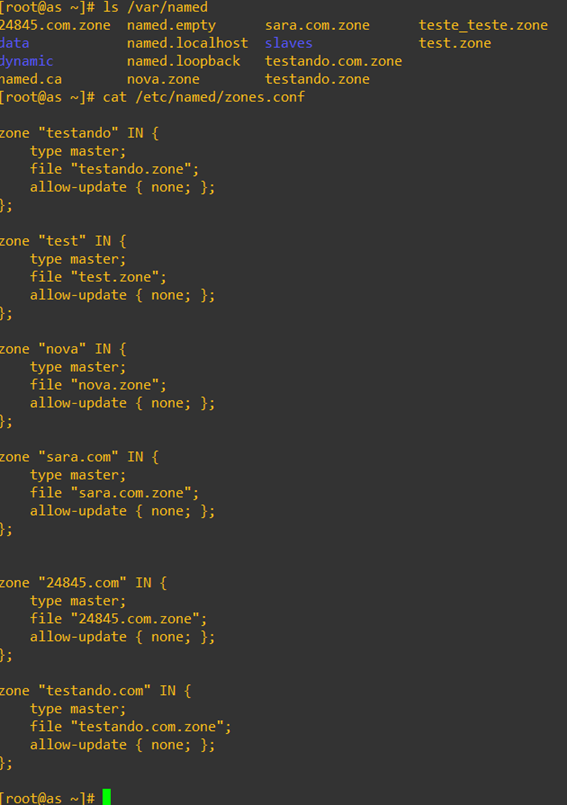
\includegraphics[width=0.78\textwidth,height=0.72\textheight,keepaspectratio]{figuras/q6_pos_named.png}
}{
  \fbox{\parbox{0.9\textwidth}{Inserir screenshot do estado final de \texttt{/var/named} e \texttt{zones.conf}.}}
}
\caption{Estado final das estruturas DNS ap\'os remo\c{c}\~ao}
\label{fig:q6-pos-named}
\end{figure}

\clearpage
\section{Quest\~ao 8: melhorias ao funcionamento da aplica\c{c}\~ao DNS}
\label{sec:q8}

\subsection{Objetivo}

A Quest\~ao 8 teve como finalidade refor\c{c}ar a aplica\c{c}\~ao desenvolvida nos pontos anteriores, introduzindo melhorias orientadas para manuten\c{c}\~ao, seguran\c{c}a operacional e robustez da configura\c{c}\~ao DNS. Em vez de acrescentar apenas uma fun\c{c}\~ao isolada, esta etapa evolui a administra\c{c}\~ao das zonas para um modelo mais seguro e mais adequado a utiliza\c{c}\~ao continuada.

As melhorias implementadas incidiram em cinco aspetos principais:
\begin{enumerate}
    \item atualiza\c{c}\~ao de registos DNS em zonas existentes;
    \item cria\c{c}\~ao autom\'atica de backups antes de altera\c{c}\~oes;
    \item reposi\c{c}\~ao da configura\c{c}\~ao anterior em caso de falha;
    \item registo das opera\c{c}\~oes em ficheiro de log;
    \item integra\c{c}\~ao das rotinas de manuten\c{c}\~ao num menu \'unico.
\end{enumerate}

\subsection{Implementa\c{c}\~ao do script \texttt{q8\_melhorias\_dns.sh}}

O script \texttt{q8\_melhorias\_dns.sh} funciona como uma camada de manuten\c{c}\~ao sobre as zonas j\'a criadas, acrescentando mecanismos de controlo que n\~ao existiam nas vers\~oes anteriores.

\begin{lstlisting}[language=bash,caption={Estrutura base, log e diretoria de backups}]
MAINCONF="/etc/named.conf"
CONFZONES="/etc/named/zones.conf"
ZONEDIR="/var/named"
LOGFILE="/var/log/projeto_dns.log"
BACKUPDIR="/root/projeto/backups_dns"

mkdir -p "$BACKUPDIR"
\end{lstlisting}

Com este bloco, a manuten\c{c}\~ao passa a ter rastreabilidade (\texttt{LOGFILE}) e recupera\c{c}\~ao (\texttt{BACKUPDIR}).

\begin{lstlisting}[language=bash,caption={Registo em log e backup automatico}]
regista_log() {
    echo "$(date '+%Y-%m-%d %H:%M:%S') - $1" >> "$LOGFILE"
}

backup_ficheiro() {
    local ficheiro="$1"
    if [ -f "$ficheiro" ]; then
        cp "$ficheiro" "$BACKUPDIR/$(basename "$ficheiro").bak.$(date +%Y%m%d%H%M%S)"
    fi
}
\end{lstlisting}

Estas fun\c{c}\~oes garantem historial das opera\c{c}\~oes e c\'opia de seguran\c{c}a antes de qualquer altera\c{c}\~ao ao ficheiro de zona.

\begin{lstlisting}[language=bash,caption={Validacao com rollback automatico}]
valida_e_aplica() {
    local dominio="$1"
    local ficheiro="$2"
    local tmpbackup="$3"

    named-checkconf >/dev/null 2>&1 || {
        regista_log "ERRO: named-checkconf falhou"
        [ -f "$tmpbackup" ] && cp "$tmpbackup" "$ficheiro"
        return 1
    }

    named-checkzone "$dominio" "$ficheiro" >/dev/null 2>&1 || {
        regista_log "ERRO: named-checkzone falhou para $dominio"
        [ -f "$tmpbackup" ] && cp "$tmpbackup" "$ficheiro"
        return 1
    }

    systemctl restart named || {
        regista_log "ERRO: restart do named falhou"
        [ -f "$tmpbackup" ] && cp "$tmpbackup" "$ficheiro"
        return 1
    }

    return 0
}
\end{lstlisting}

Este bloco introduz rollback autom\'atico: se a valida\c{c}\~ao falhar, o ficheiro volta ao estado anterior.

\begin{lstlisting}[language=bash,caption={Listagem de zonas e registos}]
listar_zonas() {
    grep '^zone "' "$CONFZONES" 2>/dev/null | awk -F'"' '{print $2}'
}

listar_registos() {
    read -p "Dominio: " DOMINIO
    ZONEFILE="$ZONEDIR/${DOMINIO}.zone"

    [ ! -f "$ZONEFILE" ] && { echo "Erro: zona nao encontrada."; return; }
    grep -E 'IN[[:space:]]+(A|MX|PTR)' "$ZONEFILE"
}
\end{lstlisting}

Estas rotinas permitem consultar o estado atual antes de alterar a zona, reduzindo erros operacionais.

\begin{lstlisting}[language=bash,caption={Adicao de registos com protecao adicional}]
adicionar_registo_a() {
    read -p "Dominio: " DOMINIO
    read -p "Host (ex: www, mail, ftp, @): " HOST
    read -p "IP: " IP

    ZONEFILE="$ZONEDIR/${DOMINIO}.zone"
    [ ! -f "$ZONEFILE" ] && { echo "Erro: zona nao encontrada."; return; }
    grep -q "^$HOST[[:space:]].*IN[[:space:]]\+A" "$ZONEFILE" && {
        echo "Erro: ja existe registo A para esse host."; return;
    }

    backup_ficheiro "$ZONEFILE"
    TMPBACKUP="/tmp/$(basename "$ZONEFILE").pre"
    cp "$ZONEFILE" "$TMPBACKUP"

    echo "$HOST    IN    A    $IP" >> "$ZONEFILE"
    atualiza_serial "$ZONEFILE"

    valida_e_aplica "$DOMINIO" "$ZONEFILE" "$TMPBACKUP" && \
    regista_log "Registo A adicionado em $DOMINIO: $HOST -> $IP"

    rm -f "$TMPBACKUP"
}
\end{lstlisting}

O fluxo aplicado aqui (backup, altera\c{c}\~ao, valida\c{c}\~ao, log) foi mantido tamb\'em nas opera\c{c}\~oes de atualiza\c{c}\~ao e remo\c{c}\~ao.

\begin{lstlisting}[language=bash,caption={Atualizacao de registos existentes}]
atualizar_registo_a() {
    read -p "Dominio: " DOMINIO
    read -p "Host do registo A a atualizar: " HOST
    read -p "Novo IP: " NOVOIP

    ZONEFILE="$ZONEDIR/${DOMINIO}.zone"
    [ ! -f "$ZONEFILE" ] && { echo "Erro: zona nao encontrada."; return; }
    grep -q "^$HOST[[:space:]].*IN[[:space:]]\+A" "$ZONEFILE" || {
        echo "Erro: registo A nao encontrado."; return;
    }

    backup_ficheiro "$ZONEFILE"
    TMPBACKUP="/tmp/$(basename "$ZONEFILE").pre"
    cp "$ZONEFILE" "$TMPBACKUP"

    sed -i "/^$HOST[[:space:]].*IN[[:space:]]\+A/c\\$HOST    IN    A    $NOVOIP" "$ZONEFILE"
    atualiza_serial "$ZONEFILE"

    valida_e_aplica "$DOMINIO" "$ZONEFILE" "$TMPBACKUP" && \
    regista_log "Registo A atualizado em $DOMINIO: $HOST -> $NOVOIP"

    rm -f "$TMPBACKUP"
}
\end{lstlisting}

\begin{lstlisting}[language=bash,caption={Remocao de registos com validacao e recuperacao}]
remover_registo() {
    read -p "Dominio: " DOMINIO
    read -p "Host a remover: " HOST
    read -p "Tipo de registo (A/MX/PTR): " TIPO

    ZONEFILE="$ZONEDIR/${DOMINIO}.zone"
    [ ! -f "$ZONEFILE" ] && { echo "Erro: zona nao encontrada."; return; }

    backup_ficheiro "$ZONEFILE"
    TMPBACKUP="/tmp/$(basename "$ZONEFILE").pre"
    cp "$ZONEFILE" "$TMPBACKUP"

    grep -v "^$HOST[[:space:]].*IN[[:space:]]\+$TIPO" "$ZONEFILE" > /tmp/zone.new
    mv /tmp/zone.new "$ZONEFILE"
    atualiza_serial "$ZONEFILE"

    valida_e_aplica "$DOMINIO" "$ZONEFILE" "$TMPBACKUP" && \
    regista_log "Registo removido em $DOMINIO: $HOST $TIPO"

    rm -f "$TMPBACKUP"
}
\end{lstlisting}

\begin{lstlisting}[language=bash,caption={Menu unificado de manutencao DNS}]
menu() {
    echo "===== MELHORIAS DNS - PONTO 8 ====="
    echo "1 - Listar zonas"
    echo "2 - Listar registos de uma zona"
    echo "3 - Adicionar registo A"
    echo "4 - Adicionar registo MX"
    echo "5 - Atualizar registo A"
    echo "6 - Atualizar registo MX"
    echo "7 - Remover registo"
    echo "8 - Ver log"
    echo "0 - Sair"
}
\end{lstlisting}

O menu centraliza as opera\c{c}\~oes e torna a manuten\c{c}\~ao mais simples no dia a dia.

\subsection{Valida\c{c}\~ao funcional}

A valida\c{c}\~ao foi feita com execu\c{c}\~ao do script e demonstra\c{c}\~ao das opera\c{c}\~oes principais: listagem, adi\c{c}\~ao, atualiza\c{c}\~ao, remo\c{c}\~ao, consulta de log e verifica\c{c}\~ao dos backups.

\begin{lstlisting}[language=bash,caption={Execucao do script}]
chmod +x /root/projeto/q8_melhorias_dns.sh
/root/projeto/q8_melhorias_dns.sh
\end{lstlisting}

\begin{lstlisting}[language=bash,caption={Verificacao do log das operacoes}]
tail -n 30 /var/log/projeto_dns.log
\end{lstlisting}

\begin{lstlisting}[language=bash,caption={Verificacao dos backups gerados}]
ls -l /root/projeto/backups_dns
\end{lstlisting}

Nos testes realizados, as opera\c{c}\~oes foram registadas corretamente e os backups foram gerados com carimbo temporal antes de cada altera\c{c}\~ao. Foi ainda poss\'ivel confirmar a manuten\c{c}\~ao de registos sem edi\c{c}\~ao manual do ficheiro de zona.

\subsection{Evid\^encias visuais da Quest\~ao 8}

\begin{figure}[!htbp]
\centering
\IfFileExists{figuras/q8_menu_listagem.png}{
  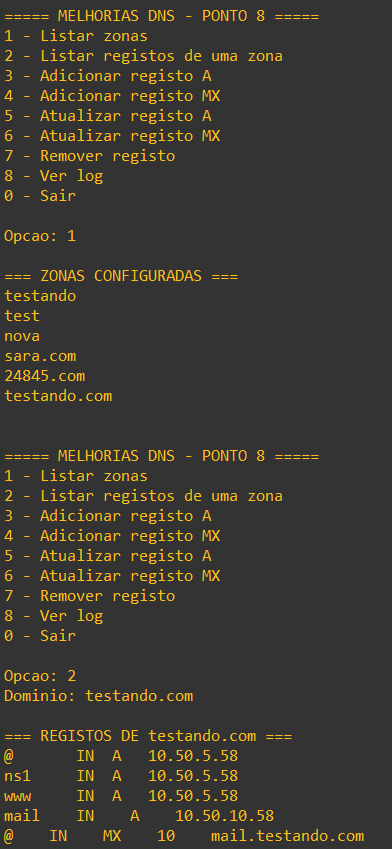
\includegraphics[width=0.78\textwidth,height=0.72\textheight,keepaspectratio]{figuras/q8_menu_listagem.png}
}{
  \fbox{\parbox{0.9\textwidth}{Inserir screenshot do menu da Quest\~ao 8 e listagem inicial de zonas/registos.}}
}
\caption{Menu da Quest\~ao 8 e listagem inicial de zonas e registos}
\label{fig:q8-menu-listagem}
\end{figure}

\begin{figure}[!htbp]
\centering
\IfFileExists{figuras/q8_add_a_mx.png}{
  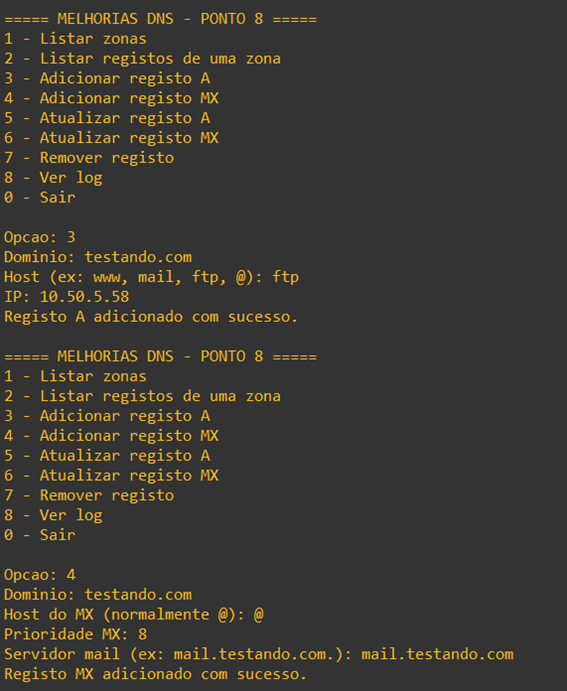
\includegraphics[width=0.78\textwidth,height=0.72\textheight,keepaspectratio]{figuras/q8_add_a_mx.png}
}{
  \fbox{\parbox{0.9\textwidth}{Inserir screenshot da adi\c{c}\~ao de registos A e MX.}}
}
\caption{Adi\c{c}\~ao de registos A e MX}
\label{fig:q8-add}
\end{figure}

\begin{figure}[!htbp]
\centering
\IfFileExists{figuras/q8_update_a_mx.png}{
  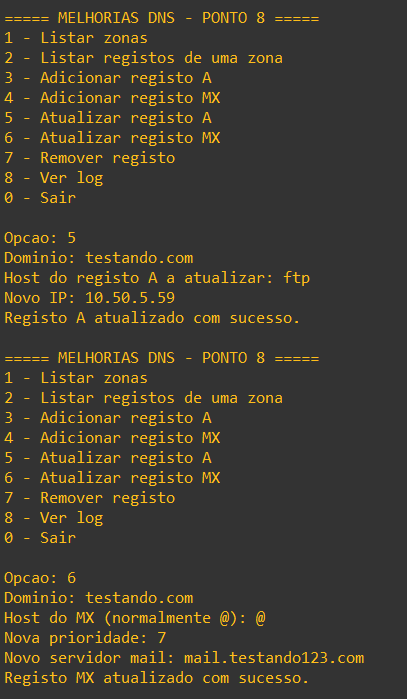
\includegraphics[width=0.78\textwidth,height=0.72\textheight,keepaspectratio]{figuras/q8_update_a_mx.png}
}{
  \fbox{\parbox{0.9\textwidth}{Inserir screenshot da atualiza\c{c}\~ao de registos A e MX.}}
}
\caption{Atualiza\c{c}\~ao de registos A e MX}
\label{fig:q8-update}
\end{figure}

\begin{figure}[!htbp]
\centering
\IfFileExists{figuras/q8_remove_log.png}{
  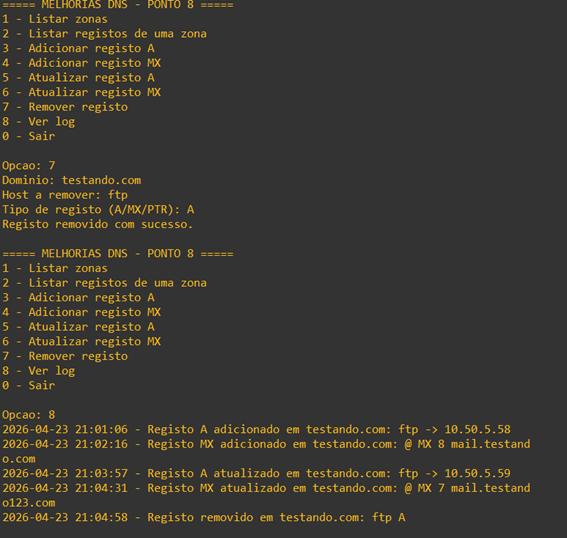
\includegraphics[width=0.78\textwidth,height=0.72\textheight,keepaspectratio]{figuras/q8_remove_log.png}
}{
  \fbox{\parbox{0.9\textwidth}{Inserir screenshot da remo\c{c}\~ao de registo e visualiza\c{c}\~ao do log.}}
}
\caption{Remo\c{c}\~ao de registos e consulta do log}
\label{fig:q8-remove-log}
\end{figure}

\begin{figure}[!htbp]
\centering
\IfFileExists{figuras/q8_listagem_final.png}{
  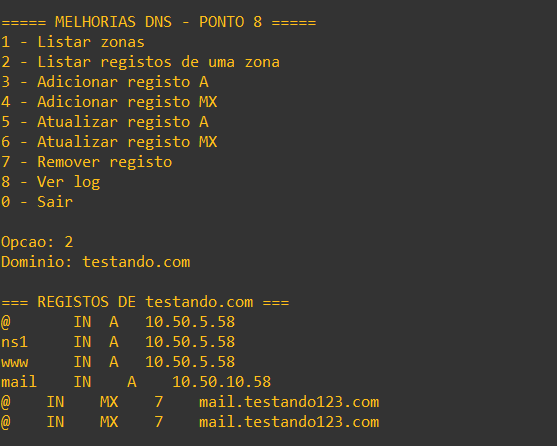
\includegraphics[width=0.78\textwidth,height=0.72\textheight,keepaspectratio]{figuras/q8_listagem_final.png}
}{
  \fbox{\parbox{0.9\textwidth}{Inserir screenshot da listagem final de registos no dom\'{\i}nio de teste.}}
}
\caption{Estado final dos registos ap\'os as opera\c{c}\~oes de manuten\c{c}\~ao}
\label{fig:q8-final}
\end{figure}

\clearpage
\section{Quest\~ao 13: cria\c{c}\~ao e gest\~ao de blacklist de dom\'inios no servidor DNS}
\label{sec:q13}

\subsection{Objetivo}

A Quest\~ao 13 teve como objetivo implementar um mecanismo de \textit{blacklist} DNS, fazendo com que dom\'inios selecionados deixem de resolver para os endere\c{c}os reais e passem a responder sempre para um IP fixo definido localmente. Para cumprir o enunciado, a solu\c{c}\~ao inclui:
\begin{enumerate}
    \item prepara\c{c}\~ao da infraestrutura de \textit{response policy} no BIND;
    \item inser\c{c}\~ao de dom\'inios na blacklist;
    \item remo\c{c}\~ao e listagem dos dom\'inios bloqueados.
\end{enumerate}

\subsection{Implementa\c{c}\~ao do script \texttt{q13\_blacklist\_dns.sh}}

O script implementa a blacklist atrav\'es de uma zona de pol\'itica de resposta (\texttt{RPZ}), designada \texttt{rpz.local}.

\begin{lstlisting}[language=bash,caption={Estrutura base da blacklist DNS}]
MAINCONF="/etc/named.conf"
CONFZONES="/etc/named/zones.conf"
RPZ_ZONE="rpz.local"
RPZ_FILE="/var/named/rpz.local.zone"
FIXED_IP="10.50.2.214"
\end{lstlisting}

Esta base separa a blacklist da configura\c{c}\~ao normal das zonas forward, mantendo a administra\c{c}\~ao mais organizada.

\begin{lstlisting}[language=bash,caption={Garantia de integracao com a configuracao DNS}]
garante_zones_conf() {
    touch "$CONFZONES"
    if ! grep -q 'include "/etc/named/zones.conf";' "$MAINCONF"; then
        echo "" >> "$MAINCONF"
        echo 'include "/etc/named/zones.conf";' >> "$MAINCONF"
    fi
}
\end{lstlisting}

\begin{lstlisting}[language=bash,caption={Criacao da configuracao base da RPZ}]
garante_rpz_config() {
    if ! grep -q 'response-policy' "$MAINCONF"; then
        awk '
        /options[[:space:]]*\{/ && done==0 {
            print
            print "        response-policy { zone \"rpz.local\"; };"
            done=1
            next
        }
        { print }
        ' "$MAINCONF" > /tmp/named.conf.new && mv /tmp/named.conf.new "$MAINCONF"
    fi

    if ! grep -q "zone \"$RPZ_ZONE\"" "$CONFZONES"; then
        cat >> "$CONFZONES" <<EOF
zone "$RPZ_ZONE" IN {
    type master;
    file "rpz.local.zone";
    allow-update { none; };
};
EOF
    fi
}
\end{lstlisting}

Este bloco ativa a diretiva \texttt{response-policy} e declara a zona \texttt{rpz.local} no BIND.

\begin{lstlisting}[language=bash,caption={Criacao do ficheiro da zona RPZ}]
if [ ! -f "$RPZ_FILE" ]; then
    SERIAL=$(date +%Y%m%d%H)
    cat > "$RPZ_FILE" <<EOF
\$TTL 86400
@   IN  SOA ns1.localhost. root.localhost. (
        $SERIAL ; serial
        3600    ; refresh
        1800    ; retry
        604800  ; expire
        86400 ) ; minimum
@       IN  NS  ns1.localhost.
ns1     IN  A   127.0.0.1
EOF
fi
\end{lstlisting}

Com a zona criada, o script passa a gerir os dom\'inios bloqueados.

\begin{lstlisting}[language=bash,caption={Insercao de dominios na blacklist}]
inserir_dominio() {
    read -p "Dominio a inserir na blacklist: " DOMINIO
    read -p "IP fixo para redirecionar [$FIXED_IP]: " IP
    [ -z "$IP" ] && IP="$FIXED_IP"

    echo "$DOMINIO     IN A    $IP" >> "$RPZ_FILE"
    echo "*.$DOMINIO   IN A    $IP" >> "$RPZ_FILE"

    atualiza_serial "$RPZ_FILE"
    validar_e_reiniciar
}
\end{lstlisting}

A fun\c{c}\~ao adiciona o dom\'inio principal e um \textit{wildcard} para subdom\'inios, garantindo bloqueio consistente.

\begin{lstlisting}[language=bash,caption={Remocao e listagem de dominios em blacklist}]
remover_dominio() {
    read -p "Dominio a remover da blacklist: " DOMINIO
    grep -Fv "$DOMINIO     IN A" "$RPZ_FILE" | \
    grep -Fv "*.$DOMINIO   IN A" > /tmp/rpz.zone.new
    mv /tmp/rpz.zone.new "$RPZ_FILE"
    atualiza_serial "$RPZ_FILE"
    validar_e_reiniciar
}

listar_blacklist() {
    grep "IN A" "$RPZ_FILE" | grep -v "ns1"
}
\end{lstlisting}

\begin{lstlisting}[language=bash,caption={Validacao e reinicio do servico}]
validar_e_reiniciar() {
    named-checkconf || { echo "Erro no named.conf"; exit 1; }
    named-checkzone "$RPZ_ZONE" "$RPZ_FILE" || { echo "Erro na zona RPZ"; exit 1; }
    systemctl restart named || { echo "Erro ao reiniciar named"; exit 1; }
}
\end{lstlisting}

\begin{lstlisting}[language=bash,caption={Menu de gestao da blacklist DNS}]
menu() {
    echo "===== MENU BLACKLIST DNS ====="
    echo "1 - Preparar configuracao RPZ/blacklist"
    echo "2 - Inserir dominio na blacklist"
    echo "3 - Remover dominio da blacklist"
    echo "4 - Listar blacklist"
    echo "0 - Sair"
}
\end{lstlisting}

\subsection{Valida\c{c}\~ao funcional}

A valida\c{c}\~ao foi realizada em quatro fases: prepara\c{c}\~ao da RPZ, teste antes da blacklist, inser\c{c}\~ao e teste ap\'os blacklist, e remo\c{c}\~ao final.

\begin{lstlisting}[language=bash,caption={Execucao inicial do script}]
chmod +x /root/projeto/q13_blacklist_dns.sh
/root/projeto/q13_blacklist_dns.sh
\end{lstlisting}

\begin{lstlisting}[language=bash,caption={Teste antes da insercao na blacklist}]
nslookup google.com 192.168.1.152
nslookup www.google.com 192.168.1.152
\end{lstlisting}

Antes da inser\c{c}\~ao, o dom\'inio respondeu com os IP reais. Depois de inserir \texttt{google.com} com redirecionamento para \texttt{192.168.1.157}, as consultas passaram a devolver esse IP fixo para \texttt{google.com} e \texttt{www.google.com}. Ap\'os remo\c{c}\~ao, a resolu\c{c}\~ao voltou ao comportamento normal.

\subsection{Evid\^encias visuais da Quest\~ao 13}

\begin{figure}[!htbp]
\centering
\IfFileExists{figuras/q13_prep_menu.png}{
  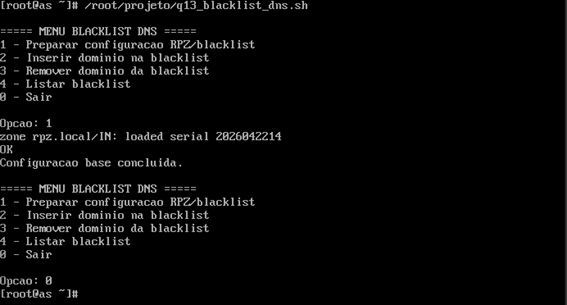
\includegraphics[width=0.78\textwidth,height=0.72\textheight,keepaspectratio]{figuras/q13_prep_menu.png}
}{
  \fbox{\parbox{0.9\textwidth}{Inserir screenshot da prepara\c{c}\~ao da configura\c{c}\~ao RPZ (op\c{c}\~ao 1).}}
}
\caption{Prepara\c{c}\~ao inicial da blacklist RPZ}
\label{fig:q13-prep}
\end{figure}

\begin{figure}[!htbp]
\centering
\IfFileExists{figuras/q13_response_policy.png}{
  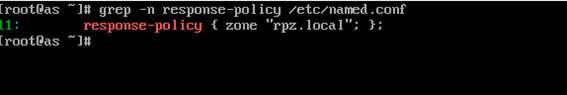
\includegraphics[width=0.78\textwidth,height=0.72\textheight,keepaspectratio]{figuras/q13_response_policy.png}
}{
  \fbox{\parbox{0.9\textwidth}{Inserir screenshot da diretiva \texttt{response-policy} no \texttt{/etc/named.conf}.}}
}
\caption{Valida\c{c}\~ao da diretiva \texttt{response-policy} no BIND}
\label{fig:q13-response-policy}
\end{figure}

\begin{figure}[!htbp]
\centering
\IfFileExists{figuras/q13_rpz_base_zone.png}{
  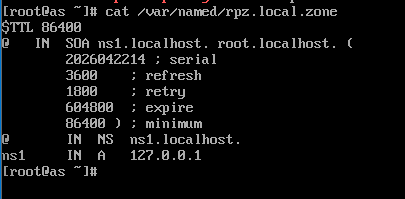
\includegraphics[width=0.78\textwidth,height=0.72\textheight,keepaspectratio]{figuras/q13_rpz_base_zone.png}
}{
  \fbox{\parbox{0.9\textwidth}{Inserir screenshot do conte\'udo inicial de \texttt{/var/named/rpz.local.zone}.}}
}
\caption{Ficheiro base da zona RPZ}
\label{fig:q13-rpz-base}
\end{figure}

\begin{figure}[!htbp]
\centering
\IfFileExists{figuras/q13_nslookup_before.png}{
  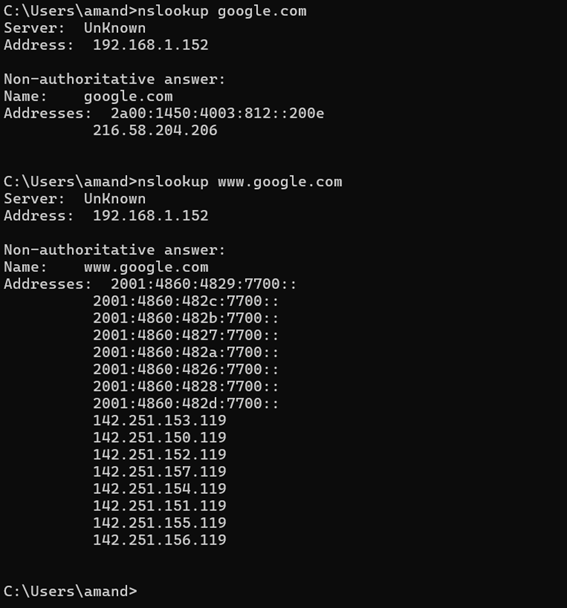
\includegraphics[width=0.78\textwidth,height=0.72\textheight,keepaspectratio]{figuras/q13_nslookup_before.png}
}{
  \fbox{\parbox{0.9\textwidth}{Inserir screenshot do \texttt{nslookup} antes da inser\c{c}\~ao na blacklist.}}
}
\caption{Resolu\c{c}\~ao normal antes da blacklist}
\label{fig:q13-before}
\end{figure}

\begin{figure}[!htbp]
\centering
\IfFileExists{figuras/q13_insert_list.png}{
  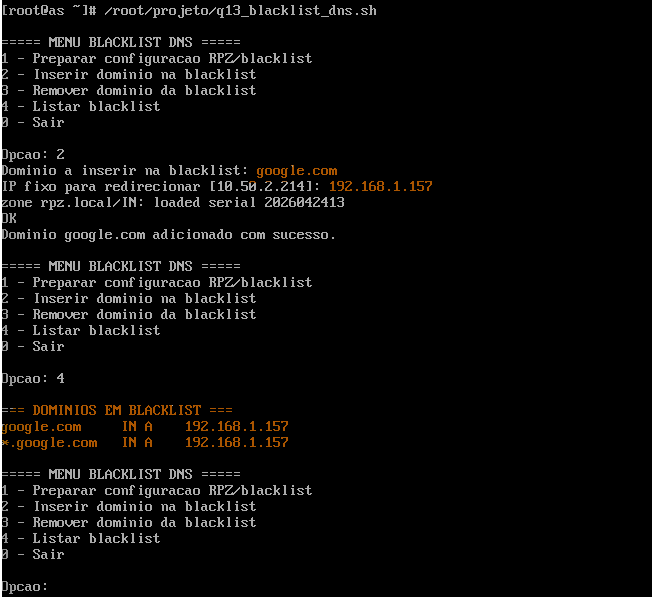
\includegraphics[width=0.78\textwidth,height=0.72\textheight,keepaspectratio]{figuras/q13_insert_list.png}
}{
  \fbox{\parbox{0.9\textwidth}{Inserir screenshot da inser\c{c}\~ao de dom\'inio e listagem da blacklist.}}
}
\caption{Inser\c{c}\~ao de \texttt{google.com} na blacklist}
\label{fig:q13-insert}
\end{figure}

\begin{figure}[!htbp]
\centering
\IfFileExists{figuras/q13_rpz_after_insert.png}{
  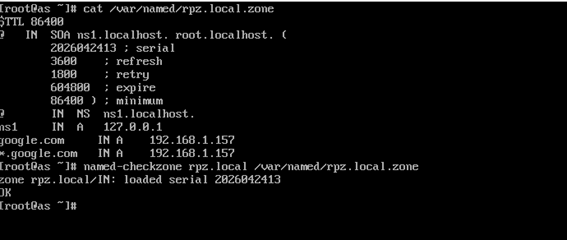
\includegraphics[width=0.78\textwidth,height=0.72\textheight,keepaspectratio]{figuras/q13_rpz_after_insert.png}
}{
  \fbox{\parbox{0.9\textwidth}{Inserir screenshot do ficheiro RPZ e valida\c{c}\~ao com \texttt{named-checkzone}.}}
}
\caption{Zona RPZ ap\'os inser\c{c}\~ao e valida\c{c}\~ao}
\label{fig:q13-zone-after}
\end{figure}

\begin{figure}[!htbp]
\centering
\IfFileExists{figuras/q13_nslookup_after.png}{
  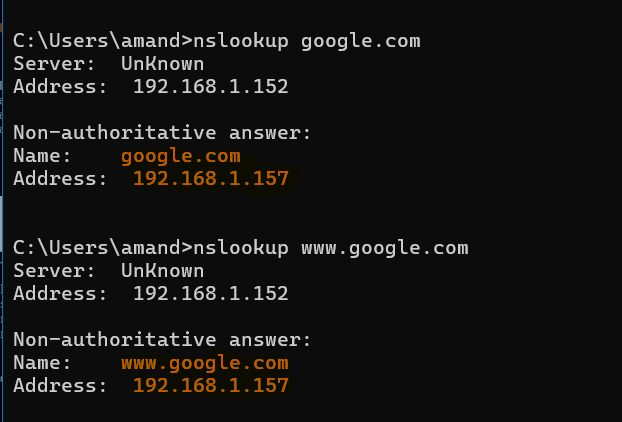
\includegraphics[width=0.78\textwidth,height=0.72\textheight,keepaspectratio]{figuras/q13_nslookup_after.png}
}{
  \fbox{\parbox{0.9\textwidth}{Inserir screenshot do \texttt{nslookup} ap\'os inser\c{c}\~ao na blacklist.}}
}
\caption{Resolu\c{c}\~ao redirecionada para IP fixo}
\label{fig:q13-after}
\end{figure}

\begin{figure}[!htbp]
\centering
\IfFileExists{figuras/q13_remove_list.png}{
  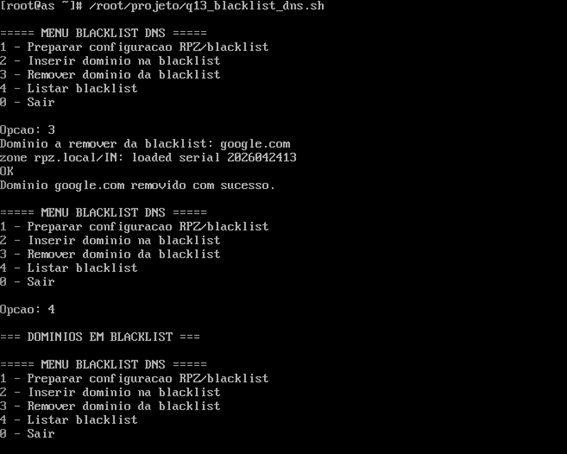
\includegraphics[width=0.78\textwidth,height=0.72\textheight,keepaspectratio]{figuras/q13_remove_list.png}
}{
  \fbox{\parbox{0.9\textwidth}{Inserir screenshot da remo\c{c}\~ao do dom\'inio e listagem final da blacklist.}}
}
\caption{Remo\c{c}\~ao do dom\'inio da blacklist}
\label{fig:q13-remove}
\end{figure}








% para adicionar o  capítulo N adicione a linha \input{capituloN} e crie o ficheiro 
% capituloN.tex na directoria "capitulos" 

%%%%%%%%%%%%%%%%%%%%%%%%%%%%%%%%%%%%%%%%%%%%%%%%
% Bibliografia
\clearpage
\thispagestyle{empty}

%\printbibliography[heading=bibintoc]
\sloppy
\printbibliography[heading=subbibliography]
\thispagestyle{empty}

%%%%%%%%%%%%%%%%%%%%%%%%%%%%%%%%%%%%%%%%%%%%%%%%
\apendices
\input{apendices/apendice1}
% para adicionar o  apêndice N adicione a linha \input{apendiceN} e crie o ficheiro 
% apendiceN.tex na directoria "apendices" 
%%%%%%%%%%%%%%%%%%%%%%%%%%%%%%%%%%%%%%%%%%%%%%%%
\anexos
\input{anexos/anexo1}
% para adicionar o  anexo N adicione a linha \input{anexoN} e crie o ficheiro 
% anexoN.tex na directoria "anexos" 
%%%%%%%%%%%%%%%%%%%%%%%%%%%%%%%%%%%%%%%%%%%%%%%%


\vfill

\SingleSpacing
{\tiny Documento elaborado com base no \ing{template for final reports and dissertations (Instituto Politécnico de Beja)}, disponível em \url{https://www.overleaf.com/project/5d936b9ea273390001434a37} para cumprimento do disposto nas"Norma para a elaboração de trabalhos académicos, produzidos no IPBeja" disponível em \url{https://www.ipbeja.pt/UnidadesOrganicas/biblioteca/Documents/NormasTrabalhosAcademicos/NormasTrabalhosAcademicos_IPBeja.pdf}.
    \version, Autor: João Paulo Barros, joao.barros@ipbeja.pt}

\end{document}

